\chapter*{Prologue: Schr\"odinger 1926--1952}
\addcontentsline{toc}{chapter}{Prologue: Schr\"odinger 1926--1952}
\markboth{PROLOGUE}{PROLOGUE}
\label{ch:prologue}

\section*{Strange or rational?}\label{sec:prologue-strange}
\index{strangeness of QM}\index{rational mechanics}

A century after its formulation, quantum mechanics is described by its own practitioners in two registers that pull in opposite directions. On one side, the empirical record:

\begin{quote}
\itshape Quantum mechanics is the most precisely tested and most successful theory in the history of science. \normalfont\hfill --- S.~Weinberg
\end{quote}

\begin{quote}
\itshape Quantum electrodynamics gives the most accurate predictions of any theory ever invented. \normalfont\hfill --- F.~Dyson
\end{quote}

\begin{quote}
\itshape All of atomic physics, molecular physics and solid-state physics are quantitatively explained by quantum mechanics with extraordinary accuracy. \normalfont\hfill --- C.~Cohen-Tannoudji
\end{quote}

On the other, the conceptual report from the same generation that built it and the one that inherited it:

\begin{quote}
\itshape The strange theory of light and matter. \normalfont\hfill --- R.~Feynman
\end{quote}

\begin{quote}
\itshape In the experiments about atomic events we have to do with things and facts, with phenomena that are just as real as any phenomena in daily life. But the atoms or elementary particles themselves are not real; they form a world of potentialities or possibilities rather than one of things or facts. This is a very strange situation. \normalfont\hfill --- W.~Heisenberg, 1958
\end{quote}

\begin{quote}
\itshape It is indeed a strange feature of quantum theory that our classical concepts are indispensable for its interpretation. \normalfont\hfill --- N.~Bohr, 1963
\end{quote}

\begin{quote}
\itshape Anyone who is not shocked by quantum theory has not understood it. If anybody says he can think about quantum physics without getting giddy, that only shows he has not understood the first thing about them. \normalfont\hfill --- N.~Bohr
\end{quote}

\begin{quote}
\itshape To me it seems like ``quantum theory'' is in a sense like a traditional herbal medicine used by ``witch doctors''. We don't REALLY understand what is happening, what the ultimate truth really is, but we have a ``cook book'' of procedures and rituals that can be used to obtain useful and practical calculations (independent of fundamental truth). \normalfont\hfill --- J.~Nash
\end{quote}

\begin{quote}
\itshape The quantum world is inexplicable in classical terms. The predictions \ldots\ governing the propagation of electromagnetic fields are in flat contradiction with the experimental facts at the microscopic scale. A key feature of quantum effects is their apparent indeterminism, that individual atomic events are unpredictable, uncontrollable and literally seem to have no cause. \normalfont\hfill --- P.~Holland, \emph{The Quantum Theory of Motion}
\end{quote}

\begin{quote}
\itshape Quantum phenomena are stranger than any fiction we could invent. \normalfont\hfill --- J.~A.~Wheeler, 1986
\end{quote}

\begin{quote}
\itshape Quantum mechanics remains the strangest of all our theories. \normalfont\hfill --- F.~Wilczek, 2014
\end{quote}

\begin{quote}
\itshape The more success the quantum theory has, the sillier it looks. \normalfont\hfill --- A.~Einstein
\end{quote}

\begin{quote}
\itshape Niels Bohr brainwashed a whole generation of theorists into thinking that the job of interpreting quantum theory was done 50 years ago. \normalfont\hfill --- M.~Gell-Mann
\end{quote}

\begin{quote}
\itshape The three biggest figures in quantum mechanics --- Schr\"odinger, Einstein and Dirac --- were all quantum skeptics. \normalfont\hfill --- R.~Penrose, 2009
\end{quote}

The transition from classical to modern physics a hundred years ago can be described as a passage from rational physics to strange physics --- where \emph{rational} means accessible to human understanding, and \emph{strange} means not. Science, by its own standards, should not be strange. The two columns of quotes above describe one and the same theory; reconciling them is the task this book takes up.

That the founders themselves were the first to call the theory strange is, in this book's reading, evidence not of nature's incomprehensibility but of an avoidable interpretational misstep. Einstein's 1935 letter to Schr\"odinger names the dynamic of that misstep with unusual clarity:

\begin{quote}
\itshape You are the only person with whom I am actually willing to come to terms. Almost all the other fellows do not look from the facts to the theory but from the theory to the facts: they cannot extricate themselves from a once accepted conceptual net, but only flop about in it in a grotesque way. \normalfont\hfill --- A.~Einstein to E.~Schr\"odinger, 1935
\end{quote}

What makes QM strange is its central object, Schr\"odinger's $N$-electron wave function
\[
\Psi(\mathbf{x}_1, \mathbf{x}_2, \ldots, \mathbf{x}_N)
\]
on a $3N$-dimensional abstract configuration space. Under Max Born's 1926 reinterpretation, $|\Psi|^2$ is a probability density for the joint configuration of all $N$ electrons. The wave function has direct physical meaning on physical 3D space only for $N=1$ (the hydrogen atom). For $N > 1$ it lives in a space of $3N$ dimensions whose physical meaning has been debated for nearly a century, and which is computationally inaccessible already for small $N$ --- representing $\Psi$ on a 100-point grid in physical space costs $O(100)$ floating-point numbers; the same grid in $3N$-dimensional space costs $O(100^N)$.

\emph{Rational physics must be computable}, because real physics evolves by performing some form of analog computation as Nature unfolds in real time. Uncomputable physics is strange physics, in a strict and not merely rhetorical sense. Nature cannot evolve a probability distribution because a probability distribution has no physical realisation; it is a mathematical object on a paper, not a state of matter.

That this is not the eccentric position of one author is acknowledged by Walter Kohn, founder of Density Functional Theory, in his 1998 Nobel Lecture:

\begin{quote}
\itshape In general the many-electron wave function $\Psi(\mathbf{x}_1, \ldots, \mathbf{x}_N)$ for a system of $N$ electrons is not a legitimate scientific concept when $N \geq N_0$, where $N_0 \approx 10^2$--$10^3$. \normalfont\hfill --- W.~Kohn, Nobel Lecture, 1998
\end{quote}

Kohn's statement is the strongest possible authoritative confirmation of the uncomputability argument: a Nobel laureate, working inside the standard formulation, declares that the central object of standard quantum mechanics ceases to be a legitimate scientific concept already at small molecular scales. Kohn's response was DFT --- a dimensional reduction. RealQM's response is a reformulation that never invokes the $3N$-dimensional object in the first place.

That standard QM works at all is due to a sequence of drastic dimensional reductions of $\Psi$ to objects that \emph{are} computable and that \emph{do} have direct meaning on 3D space --- a sequence of \textbf{rescue attempts}, in fact, each one responding to the uncomputability of the unreduced $\Psi$: Thomas--Fermi (1930) replaces the wave function by an electron density and gives up electron individuality; Hartree--Fock (1930s) restores individuality through Slater determinants of one-electron orbitals at the cost of an ad hoc antisymmetric ansatz; Density Functional Theory (1980s, Kohn--Sham), the working tool of computational chemistry, returns to a single electron density $\rho(\mathbf{x})$ on $\mathbb{R}^3$ supplemented by an exchange-correlation functional whose exact form is unknown; and Bader's \emph{Atoms in Molecules}~\cite{Bader90} partitions that 3D density into atomic basins via zero-flux surfaces of $\nabla\rho$, recovering a real-space picture of distinct electronic territories as a post-processing step on top of a Slater-determinant density. Each rescue attempt delivers the empirical success the practitioners praise; the unreduced $\Psi$ is what they call strange. RealQM continues the same direction --- back to 3D, back to computable objects, back to electronic territories with the same zero-flux/homogeneous-Neumann boundary condition that AIM uses --- but from the foundations rather than as a post-hoc workaround on top of a $3N$-dimensional formulation that was never tractable in the first place. The Bader partition, in particular, is built into RealQM as the primary variational object rather than extracted from a StdQM density afterwards.

RealQM, the framework developed in this book, proposes a refinement in the same direction as DFT but starting from the foundations: a set of $N$ non-overlapping one-electron charge densities $\psi_i^2$ on a partition of physical 3D space, with the configuration-space step never taken. It is computable from the start. The rational ingredients of Schr\"odinger's 1926 equation --- Coulomb interaction between charge densities, a measure of electron compression in the gradient $|\nabla \psi_i|^2$ --- are kept; the strange ingredients --- the $3N$-dimensional configuration space, the probabilistic reinterpretation --- are removed. The result is a form of rational mechanics, in the older sense of the term: an equation that can be written down, solved on a laptop, and checked against experiment without an interpretational layer.

\bigskip
\hrule
\bigskip

\section*{Schr\"odinger as protagonist}\label{sec:prologue-protagonist}

The central figure of this book is Erwin Schr\"odinger. His wave equation of early 1926 gave physics its working tool for atomic matter and chemistry, and his lifelong objection --- restated explicitly in his Dublin Colloquium of 1952 --- maintained that the historical reinterpretation of the wave function in 1926--1929 as a probability density on $3N$-dimensional configuration space was a wrong turn. The 26 years between 1926 and 1952 frame the conceptual arc of this Prologue. The cast that drove that arc --- Planck, Bohr, Schr\"odinger himself, Heisenberg, Born, Dirac --- is introduced below in compact form.

\paragraph{Planck, 1900: the quantum.}
The thread begins with Max Planck's analysis of black-body radiation. To fit the observed spectrum, Planck postulated that the exchange of energy between matter and radiation could occur only in discrete amounts $E = h\nu$, with $h$ a new fundamental constant. The postulate was reluctant on Planck's part and was not initially read as a statement about the nature of matter; it was a device for closing a thermodynamic argument --- Planck himself later described it as a formal assumption introduced under pressure, an act of desperation undertaken because no classical derivation of the observed spectrum had worked. He spent much of the following decade attempting to recover the spectrum without the quantum hypothesis, in a series of papers (the ``second theory,'' 1911--1914) trying to make absorption continuous while keeping emission discrete; none of these attempts succeeded, and the quantum hypothesis remained in the literature as the only working derivation. Within a few years it had become the seed of a much larger story. Planck himself never embraced that story: when the probabilistic interpretation of quantum mechanics took shape in the late 1920s, he sided with Einstein against the Copenhagen reading and remained, to his death in 1947, a defender of classical determinism and continuous physical processes. The founder of the quantum era was uneasy with his own founding step from the day he took it, and uneasy with the theory built on top of it for the rest of his life.

\paragraph{Bohr, 1913: the atom with discrete orbits.}
Niels Bohr applied Planck's quantum to atomic structure: the hydrogen atom was described as an electron in one of a discrete set of allowed circular orbits around a positive kernel, with transitions between orbits accompanied by emission or absorption of a photon of the corresponding energy. The Bohr model reproduced the hydrogen spectrum to remarkable accuracy and gave the periodic table its first quantitative anchor. It was, however, internally inconsistent: an orbiting electron should radiate continuously and spiral into the nucleus, and the model's quantisation of angular momentum was imposed externally rather than derived. The Bohr model worked, in a way no one could quite explain.

\paragraph{Schr\"odinger, 1926: the wave equation in real 3D space.}
In early 1926, Erwin Schr\"odinger published the equation that became the working framework of atomic physics and chemistry: a wave equation for a real-valued function $\psi(\mathbf{x})$ on physical 3D space, with $\psi^2$ representing the electron's charge density. For hydrogen, the equation
\[
-\tfrac{1}{2}\Delta \psi - \frac{\psi}{|\mathbf{x}|} \;=\; E\, \psi
\]
had stationary solutions whose eigenvalues reproduced the hydrogen spectrum exactly. Schr\"odinger had been working with de Broglie's idea of matter waves and had been searching for the partial differential equation those waves should satisfy. The hydrogen solution was found in the Alps during a sustained burst of creative work in late 1925 and early 1926. The wave function lived in physical 3D space; $\psi^2$ was an electron charge density in the same sense as Maxwell's $\rho$ is an electromagnetic charge density. The framework was a working tool for chemists and physicists almost immediately. \emph{This wave equation, in its real-3D-space form, is the foundation of this book.}

\paragraph{Heisenberg, 1925: matrix mechanics (the alternative algebraic framework).}
A few months earlier, in mid-1925, Werner Heisenberg --- working with Max Born and Pascual Jordan --- had proposed a different mathematical framework: the observables of an atomic system represented by non-commuting matrices indexed by the system's stationary states, with the time evolution governed by what came to be called the Heisenberg equation. Matrix mechanics dispensed with the orbits and trajectories of the Bohr picture entirely; the hydrogen spectrum and selection rules emerged from the algebra of the matrices. It was abstract in a way that physicists trained on differential equations found difficult to use as a working tool. The equivalence of matrix mechanics and Schr\"odinger's wave mechanics was established within months by Schr\"odinger, Dirac, and others --- the two formalisms gave the same predictions for hydrogen and for the simplest multi-electron systems. From the perspective of 1926, physics had been handed two formulations of the same theory: one algebraic, one in real 3D space.

\paragraph{Born, 1926: the probabilistic interpretation.}
Max Born then proposed the move that defined modern atomic physics. For the multi-electron case, Born argued, the natural object was a single wave function $\Psi(\mathbf{x}_1, \ldots, \mathbf{x}_N)$ on the $3N$-dimensional product space, with $|\Psi|^2$ a joint \emph{probability} density: the probability that, upon measurement, the system is found in the configuration with electron~1 at $\mathbf{x}_1$, electron~2 at $\mathbf{x}_2$, and so on. Marginal one-electron densities arose by integration over the other coordinates; expectation values arose by integration against operators. Born's interpretation gave wave mechanics a working calculation framework for scattering and for many-electron systems and was rapidly adopted as the standard reading. The price, on Schr\"odinger's reading, was that the wave function was no longer a physical field on physical space; it was a mathematical device for computing probabilities, and the configuration-space wave function had no physical meaning on $\mathbb{R}^3$ for $N > 1$.

\paragraph{Schr\"odinger at Solvay, 1927: the contested choice point.}\label{par:solvay-1927}\index{Solvay Conference, 1927}
The 5th Solvay Conference of October 1927, often remembered as the moment at which the configuration-space-plus-probability reading became the standard formulation, was in fact a meeting at which sharply conflicting interpretations were defended in parallel --- de Broglie's pilot-wave theory,\footnote{It was de Broglie himself who introduced the pilot wave (\emph{onde pilote}), in his communication to this 1927 Solvay Conference, as the reduced form of his \emph{th\'eorie de la double solution}. This is a separate proposal from his 1924 matter-wave hypothesis (the $\lambda = h/p$ relation on which Schr\"odinger built): the matter wave is a wave \emph{associated with} the particle, whereas the pilot wave is a real wave that \emph{guides} a localised particle along definite trajectories. After criticism at Solvay --- notably Pauli's objection on the inelastic scattering of a particle by a rotator --- de Broglie abandoned the theory; it was independently rediscovered and completed as a consistent hidden-variable theory by David Bohm in 1952, and is now known as the de Broglie--Bohm theory. The pilot-wave idea is thus de Broglie's, not Bohm's alone.} Born and Heisenberg's matrix mechanics with the probabilistic interpretation, and Schr\"odinger's wave mechanics on real 3D space. Schr\"odinger used the Solvay platform to argue for a programmatic 3D-space alternative to the configuration-space extension, and his statement at Solvay is, in this book's reading, the documentary anchor for the RealQM construction. From Schr\"odinger's Solvay 1927 communication:
\begin{quote}
\itshape The attempts to derive numerical results by means of approximation methods for the atom with several electrons, whose amplitude equation or wave equation cannot be solved directly, have led to the remarkable result that actually, despite the multi-dimensionality of the original equation, in this procedure one always needs to calculate only with the well-known three-dimensional eigenfunctions of hydrogen; indeed one has to calculate certain three-dimensional charge distributions that result from the hydrogen eigenfunctions according to the principles presented above, and one has to calculate according to the principles of classical electrostatics the self-potentials and interaction potentials of these charge distributions \ldots\ Herein, I think, lies a hint that with the furthering of our understanding ``in the end everything will indeed become intelligible in three dimensions again.'' \normalfont\hfill --- E.~Schr\"odinger, Solvay Conference, October 1927
\end{quote}
This is, almost line for line, the RealQM construction: real one-electron charge densities on physical 3D space, interacting through classical electrostatic self- and mutual potentials. Schr\"odinger sketched the programme; Bohr, Born, and Heisenberg argued against it; the room went the other way. The framework developed in the present book is the carrying-out, with the benefit of a century of accumulated experience and the computational tools the original participants did not have, of the programme Schr\"odinger outlined that week.

\paragraph{Dirac, 1929: chemistry as applied physics.}
Paul Dirac's transformation theory unified Born's probabilistic reading with Heisenberg's matrix mechanics and Schr\"odinger's wave equation into a single framework. By the 5th Solvay Conference in 1927, the configuration-space-plus-probability framework had become the standard formulation; by Dirac's 1929 declaration that ``the underlying physical laws necessary for the mathematical theory of \ldots\ the whole of chemistry are thus completely known, and the difficulty is only that the exact application of these laws leads to equations much too complicated to be soluble'', it was the foundation of modern atomic physics. The Schr\"odinger equation in $3N$-dimensional configuration space, with antisymmetric wave functions and Born's probabilistic interpretation, has been the working theory of the field ever since. \emph{Dirac's sentence is the chapter epigraph for this book's central technical claim: the underlying physics is known; the equations are merely too complicated. A different formulation that is not too complicated, working in real 3D space throughout, is the subject of what follows.}

\paragraph{What the choice cost.}
The configuration-space extension was decisive but expensive. Schr\"odinger's original 3D-space interpretation, in which $\psi^2$ was a literal charge density, was abandoned in favour of a probability density on a $3N$-dimensional abstract space whose physical meaning has been debated for nearly a century. The computational cost grew exponentially in $N$: representing $\Psi$ on a 100-point grid in physical space costs $O(100)$; the same grid in $3N$-dimensional space costs $O(100^N)$. Every quantum chemistry method developed since 1929 --- Hartree--Fock, configuration interaction, coupled cluster, density functional theory --- is a strategy for managing this exponential cost. The chemistry-specific machinery of those methods (basis sets, exchange--correlation functionals, pseudopotentials, dispersion corrections) emerged because the configuration-space equation could not be solved directly.

Schr\"odinger himself never accepted the probabilistic interpretation, and the historical record contains many reminders of his persistent objection. Two of them appear in Chapter~\ref{ch:dirac} when we elaborate the configuration-space step; more are scattered through later chapters. Pauli's own assessment of the antisymmetry postulate --- which he could not derive and considered a ``deficiency'' even on the occasion of receiving the 1945 Nobel Prize for it --- is taken up in Chapter~\ref{ch:equation}, where antisymmetry is replaced by spatial non-overlap.

\paragraph{RealQM: a return to Schr\"odinger in 3D.}
This book is built around the proposition that the choice made in 1926--1929 was the wrong choice --- and that Schr\"odinger, who maintained this objection from March 1926 through to his Dublin Colloquium of 1952, was right. The formulation developed here, which we call \textbf{RealQM}, returns to the real-3D-space picture that Schr\"odinger originally envisaged. The $N$-electron wave function $\Psi(\mathbf{x}) = \sum_{i=1}^N \psi_i(\mathbf{x})$ lives on physical $\mathbb{R}^3$ as a sum of one-electron wave functions on a non-overlapping partition of space. Each $\psi_i^2$ is an actual charge density. The configuration-space step is not taken at all.

The price paid for staying in 3D is the replacement of antisymmetry with strict spatial non-overlap of the one-electron supports. The two requirements are not equivalent, and the resulting framework is a different mathematical object from standard quantum mechanics rather than a numerical approximation of it. The benefit is that the computational obstacle Dirac identified --- equations too complicated to be soluble --- is dissolved. The framework fits in 8000 lines of code and runs interactively on a laptop GPU.

\paragraph{How to read the rest of the book.}
Chapter~\ref{ch:dirac} elaborates the choice point of 1926--1929, frames the two foundational positions on it (Dirac's and the Copenhagen interpretation's), and previews the alternative the book develops. Chapter~\ref{ch:equation} writes down RealSE, the Real Schr\"odinger Equation, derives its Euler--Lagrange equations, and identifies the free-boundary condition that closes the system. Chapter~\ref{ch:hierarchy} sets out the four levels of reduction. Part~II describes how the equations are solved. Part~III works through the validation across atoms, molecules, reactions, folding, and condensed phases. Part~IV returns to foundational questions --- stability of matter and the nuclear-scale extension --- in light of the validation. Part~V places the framework in its broader context: chemistry vs.\ physics, and the human--AI collaboration through which the work was carried out.

\textbf{The book is best read complementing the text by running and modifying the codes in the Gallery on GitHub.} Every quantitative claim in the book corresponds to a runnable simulation; static prose can describe \emph{what} is computed, but the Gallery lets the reader \emph{run} the code, \emph{change} a parameter, and watch the chemistry respond live in a browser window. Each chapter of Part~III has corresponding Gallery cards listed in the Appendix. A modern browser and a few minutes of setup are all that is needed; nothing in the framework requires installation, compilation, or a remote service.

\bigskip
\hrule
\bigskip

\section*{Interlude: Schr\"odinger in Copenhagen, autumn 1926}

A short historical vignette closes the Prologue, because it captures the human dimension of the choice point that the rest of the book is about.

In September 1926, shortly after the publication of the wave equation, Niels Bohr invited Erwin Schr\"odinger to Copenhagen. Schr\"odinger travelled to Bohr's institute expecting a discussion among colleagues about the new wave mechanics; what he encountered was something rather different. Bohr met him at the train station and began arguing immediately. The arguments continued at Bohr's house, where Schr\"odinger was a guest, with Bohr pressing his case against Schr\"odinger's real-space interpretation of $\psi^2$ and in favour of the probabilistic, complementarity-driven reading then taking shape in Copenhagen.

Werner Heisenberg, present in Copenhagen and observing the exchange first-hand, recorded the intensity of the encounter in his memoir:

\begin{quote}
The discussion between Bohr and Schr\"odinger began at the railway station in Copenhagen and was carried out every day from early morning to late night. Bohr appeared to me like a relentless fanatic, who was not prepared to concede a single point to his interlocutor or to allow him the slightest lack of precision. It will scarcely be possible to reproduce how passionate the discussion was carried out from both sides.\\
\hfill --- W.~Heisenberg, \emph{Der Teil und das Ganze}, 1969.
\end{quote}

After several days of unrelenting debate Schr\"odinger fell ill and took to bed at the Bohr residence. Bohr, by Heisenberg's account, sat at the bedside and continued the argument while Mrs Bohr brought tea and pastries. Schr\"odinger eventually returned to Z\"urich exhausted and is reported to have said, in the immediate aftermath:

\begin{quote}
If we are still going to have to put up with these damned quantum jumps, I am sorry that I ever had anything to do with quantum mechanics.\\
\hfill --- Schr\"odinger to Bohr, 1926.
\end{quote}

He never accepted the probabilistic interpretation. He went on writing about the issue --- the cat-paradox paper of 1935, the letter to Einstein in 1950, the Dublin lectures of 1952 --- for the rest of his life. In private correspondence and conversation he was less guarded than in print, and the historical record preserves several characterisations of the Copenhagen consensus in his own voice:

\begin{quote}
\itshape With very few exceptions (such as Einstein and Laue), all the rest of the theoretical physicists were unadulterated asses and I was the only sane person left. The one great dilemma that ails us day and night is the wave-particle dilemma.
\end{quote}

\begin{quote}
\itshape If I were not thoroughly convinced that the man [Bohr] is honest and really believes in the relevance of his --- I do not say theory but sounding word --- I would call it intellectually wicked.
\end{quote}

\begin{quote}
\itshape So unable is the good average physicist to believe that any sound person could refuse to accept the Copenhagen oracle.
\end{quote}

The choice point of 1926 was, from his side, never closed; from the side of the Copenhagen interpretation, it was closed during this very visit. Modern atomic physics was shaped at Bohr's house in autumn 1926, with one of the founders of the field on the sofa, ill and overpowered.

\begin{figure}[h]
\centering
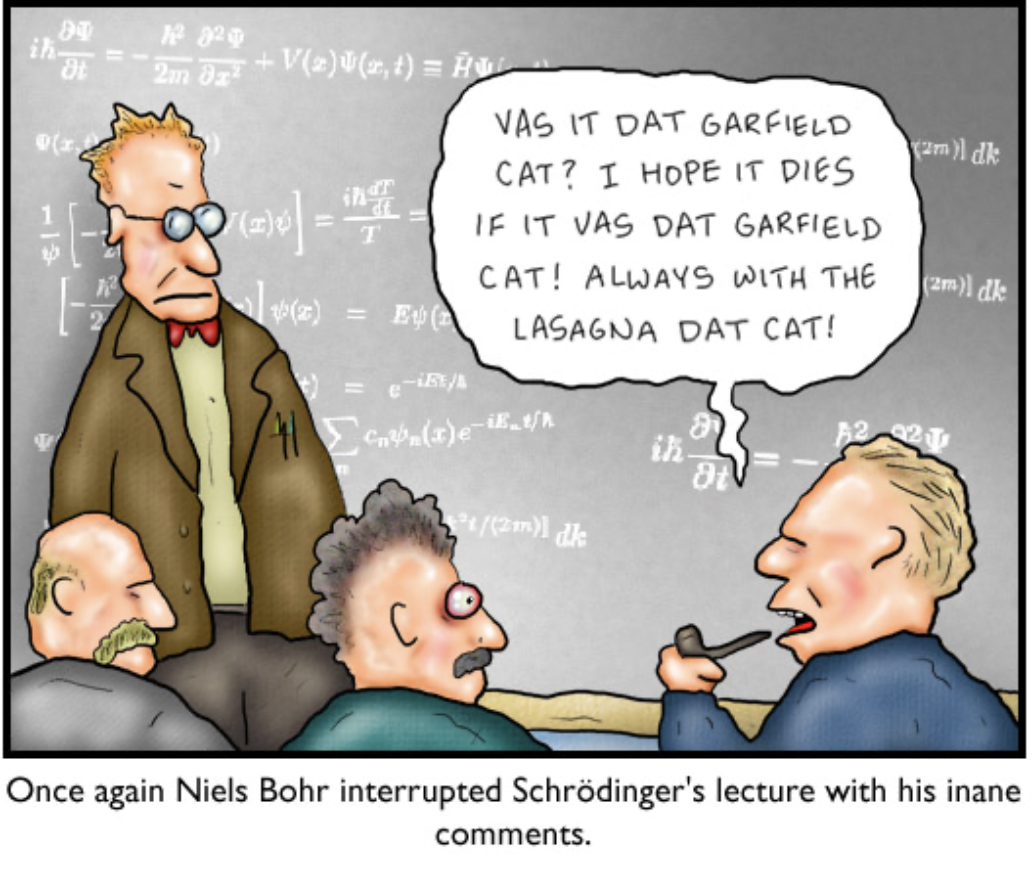
\includegraphics[width=0.55\textwidth]{pictures/bohrschrodinger.png}
\caption{A Larson cartoon recalling Schr\"odinger's Copenhagen experience: ``Once again Niels Bohr interrupted Schr\"odinger's lecture with his inane comments.''}
\end{figure}

\bigskip
\hrule
\bigskip

\section*{Coda: Dublin, 1952}\label{sec:prologue-dublin}

Twenty-six years after the Copenhagen visit, at a Colloquium in Dublin, Schr\"odinger restated his position. The conviction he had carried since March 1926 had not softened. The Bohr--Born--Heisenberg reading that had been adopted then as the Copenhagen interpretation, and which had filled the textbooks and the minds of students and physicists in the meantime, was --- in his judgement --- still the wrong turn.\index{Dublin Colloquium, 1952}

\begin{quote}
Let me say at the outset that, in this discourse, I am opposing not a few special statements of quantum mechanics held today; I am opposing as it were the whole of it, I am opposing its basic views that have been shaped 25 years ago, when Max Born put forward his probability interpretation, which was accepted by almost everybody. It has been worked out in great detail to form a scheme of admirable logical consistency that has been inculcated ever since to every young student of theoretical physics.

The view I am opposing is so widely accepted, without ever being questioned, that I would have some difficulties in making you believe that I really, really consider it inadequate and wish to abandon it.

It is, as I said, the probability view of quantum mechanics. You know how it pervades the whole system. It is always implied in everything a quantum theorist tells you. Nearly every result he pronounces is about the probability of this or that or that\ldots\ happening --- with usually a great many alternatives. The idea that they be not alternatives but all really happen simultaneously seems lunatic to him, just impossible. He thinks that if the laws of nature took this form for, let me say, a quarter of an hour, we should find our surroundings rapidly turning into a quagmire, or sort of a featureless jelly or plasma, all contours becoming blurred, we ourselves probably becoming jellyfish.

It is strange that he should believe this. For I understand he grants that unobserved nature does behave this way --- namely according to the wave equation. The aforesaid alternatives come into play only when we make an observation, which need, of course, not be a scientific observation. Still it would seem that, according to the quantum theorist, nature is prevented from rapid jellification only by our perceiving or observing it. And I wonder that he is not afraid, when he puts a ten-pound note (or his wrist-watch) into his drawer in the evening, he might find it dissolved in the morning, because he has not kept watching it.\\
\hfill --- E.~Schr\"odinger, Dublin Colloquium, 1952.
\end{quote}

The objection is not subtle. A theory whose predictions are statistical statements about \emph{what might be observed} requires a physical world that does not exist independently of the observation. Schr\"odinger considered this a structural failure of the formulation, not a feature of the physics. His position never softened.

Two further passages from the same period (published in \emph{The Interpretation of Quantum Physics}, Ox Bow Press, Woodbridge CN, 1995) make the positive content of his alternative more explicit. The first is the ontology that the Dublin remarks defend; the second is the philosophical stake:

\begin{quote}
\itshape What we observe as material bodies and forces are nothing but shapes and variations in the structure of space. Particles are just schaumkommen (appearances). \normalfont\hfill --- E.~Schr\"odinger
\end{quote}

\begin{quote}
\itshape It has been doubted whether atomic events can even be described in the space-time form of thought. From the philosophical standpoint, I would consider a definite decision of this sort to be equivalent to complete surrender. \normalfont\hfill --- E.~Schr\"odinger
\end{quote}

The first passage is the closest concise statement in Schr\"odinger's own voice of what RealQM constructs technically: matter as a continuum density distribution on physical 3D space, with particles as visible features (\emph{Schaumkommen}, foam-appearances) of that underlying continuum rather than as primary ontological constituents. The second states the philosophical stake: to give up the space-time form of description for atomic events would be ``complete surrender'' --- exactly what the configuration-space step of 1926--1929, with the wave function transferred to $\mathbb{R}^{3N}$ and reinterpreted as a probability density, did. This book is, in the literal sense, a refusal of that surrender.

A third remark, in the same vein, addresses the role of idealised single-particle reasoning in the foundational discussions of QM:

\begin{quote}
\itshape We never experiment with single electrons, atoms or small molecules. In thought experiments we assume we do. It always results in ridiculous consequences. \normalfont\hfill --- E.~Schr\"odinger
\end{quote}

The thought-experiment apparatus that has carried much of the conceptual debate of QM --- single particles passing through single slits, single electrons in superposed states, single observers making single measurements --- is not, on Schr\"odinger's reading, the regime in which the theory actually does its empirical work. The theory's empirical successes are statistical statements about ensembles of many atoms; the foundational paradoxes attach to idealisations that real experiments never realise. The point will recur in later chapters.

\paragraph{The book's position on statistics.}
This book takes Schr\"odinger's side on the 1926 choice point. Each $\psi_i^2(\mathbf{x})$ on $\Omega_i \subset \mathbb{R}^3$ is the actual electronic charge density of electron $i$ in that region of space, in the same sense that Maxwell's $\rho(\mathbf{x})$ is the electromagnetic charge density. The variational principle of Chapter~\ref{ch:equation} picks out the configuration the system occupies; the prediction is a deterministic statement about that configuration.

Statistics enters physics where the situation is genuinely an ensemble: in thermodynamics (which Body and Soul Vol~5~\cite{BodyAndSoulV} develops as a deterministic continuum theory, without statistical-mechanical ensembles as a primary ingredient); in experimental measurement noise; in many-body simulations where many configurations are sampled in time. It does not enter the description of a single isolated quantum system. The two volumes together --- Vol~5 for macroscopic thermodynamics, the present volume for atomic-scale matter --- are intended to offer a deterministic continuum-mechanics treatment of physics from macroscopic to atomic scales, in the Body and Soul tradition, in the spirit of Schr\"odinger's Dublin remarks.

\bigskip

The rest of this book is an attempt to revisit, with the benefit of a century of accumulated experience and the practical tools the original participants did not have, the choice that the autumn 1926 visit consolidated and that Schr\"odinger contested for the rest of his life.

\bigskip
\begin{figure}[h]
\centering
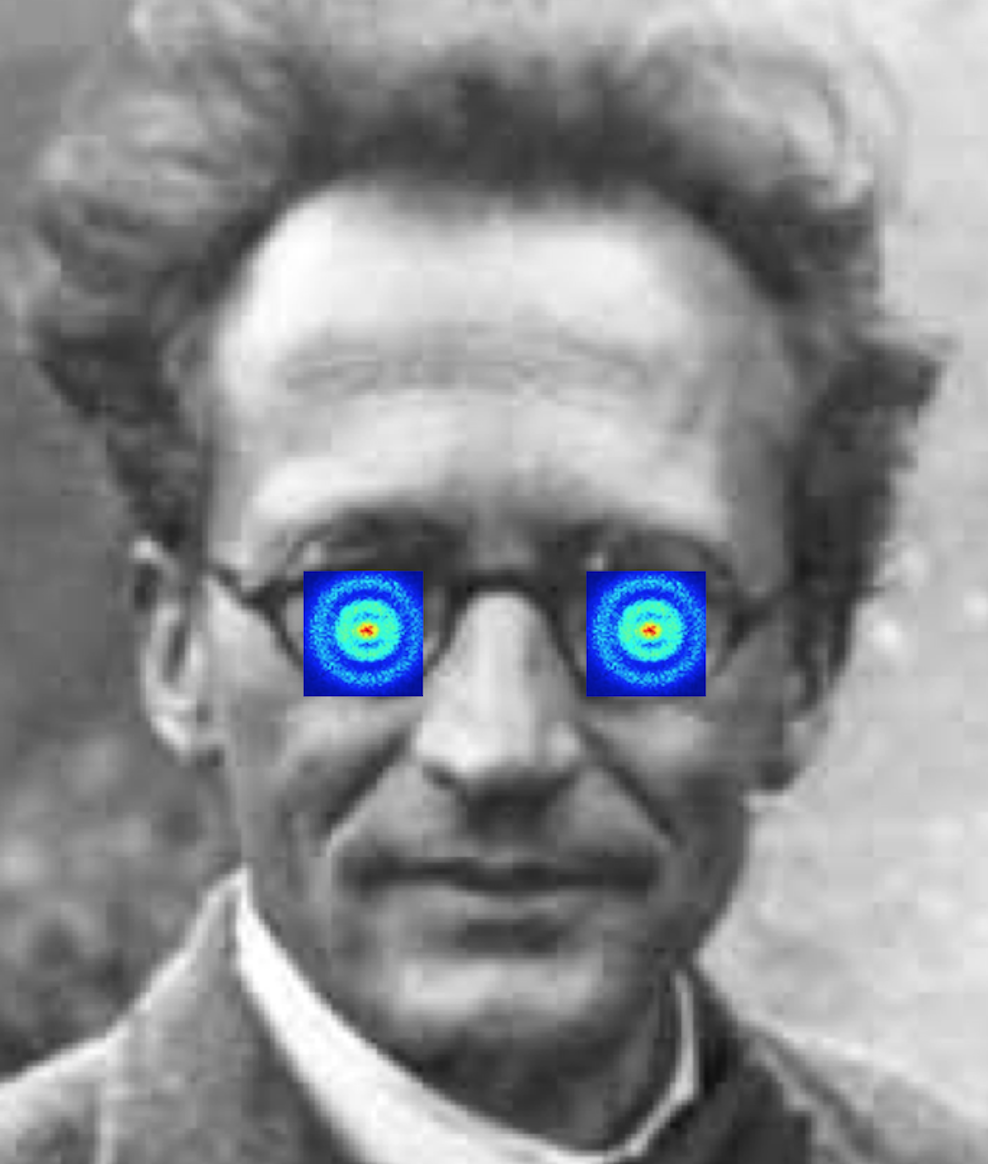
\includegraphics[width=0.55\textwidth]{pictures/schrodinger100.png}
\caption{Erwin Schr\"odinger (1887--1961). The wave equation of 1926 and the Dublin lectures of 1952 bracket the conceptual arc of this Prologue.}
\end{figure}

% --- End of Prologue ---
